\documentclass{report}
\usepackage{graphicx} % Required for inserting images
\usepackage[italian]{babel}
\usepackage{tikz}
\usepackage{hyperref}
\usepackage{amsmath}
\usepackage{xcolor}
\usepackage{float}
\usepackage{soul}
\usepackage{listings} % Per evidenziare il codice

\definecolor{lightgray}{rgb}{0.9,0.9,0.9} % Definizione colore sfondo
\definecolor{darkgreen}{rgb}{0.0, 0.5, 0.0}

\lstset{
    backgroundcolor=\color{lightgray}, % Sfondo grigio
    basicstyle=\ttfamily, % Font monospaziato
    % frame=single, % Bordo attorno al codice
    tabsize=4, % Dimensione tabulazione
    breaklines=true, % Permette di andare a capo automaticamente
    numbers = left,
    numberstyle=\small\color{gray}
}

\title{\huge\textbf{{Modellazione e Analisi di Sistemi}}}
\date{}

\begin{document}

\maketitle

\tableofcontents
\newpage

\chapter{Abstract State Machines}

Le ASM sono delle FSM (\textit{Final State Machines}) con stati generalizzati; rappresentano la forma 
matematica di macchine che estendono la nozione di FSM, \textbf{ampliando la definzione di stato} 
e \textbf{modificando la forma delle transizioni}.

\subsubsection{Stati}
Gli stati di controllo non strutturati vengono sostituiti da stati (strutturati) che 
modellano:
\begin{itemize}
    \item \textbf{dati} complessi arbitrati (con domini di base e funzioni per la struttura)
    \item \textbf{operazioni} per la manipolazione di dati
\end{itemize}

\noindent Possiamo definire gli stati come delle \textit{algebre}.

\begin{figure}[H]
    \centering
    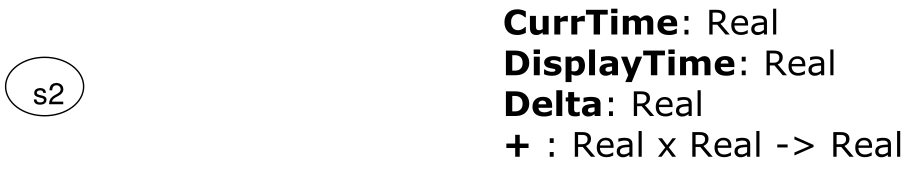
\includegraphics[width=0.8\linewidth]{chapters/1-asm/images/stati.png}
\end{figure}

\subsubsection{Transizioni}
Le transizione sono \textit{"regole"} che descrivono il cambiamento 
di funzioni da uno stato al successivo; permettono di modificare la 
struttura algebrica durante l'esecuzione della ASM.

\begin{center}
    \textit{if condition then Updates}
\end{center}

\noindent Negli FSM le transizioni sono rappresentate con delle frecce.

\newpage
Le ASM sono dotate di un ambiente di tool per:
\begin{itemize}
    \item editing
    \item simulazione
    \item validazione 
    \item verifica
    \item generazioni di casi di test
\end{itemize}

\noindent Un modello ASM può essere visto come pseudocodice su strutture dati astratte.

\subsubsection{Da FSM a ASM}
\begin{figure}[H]
    \centering
    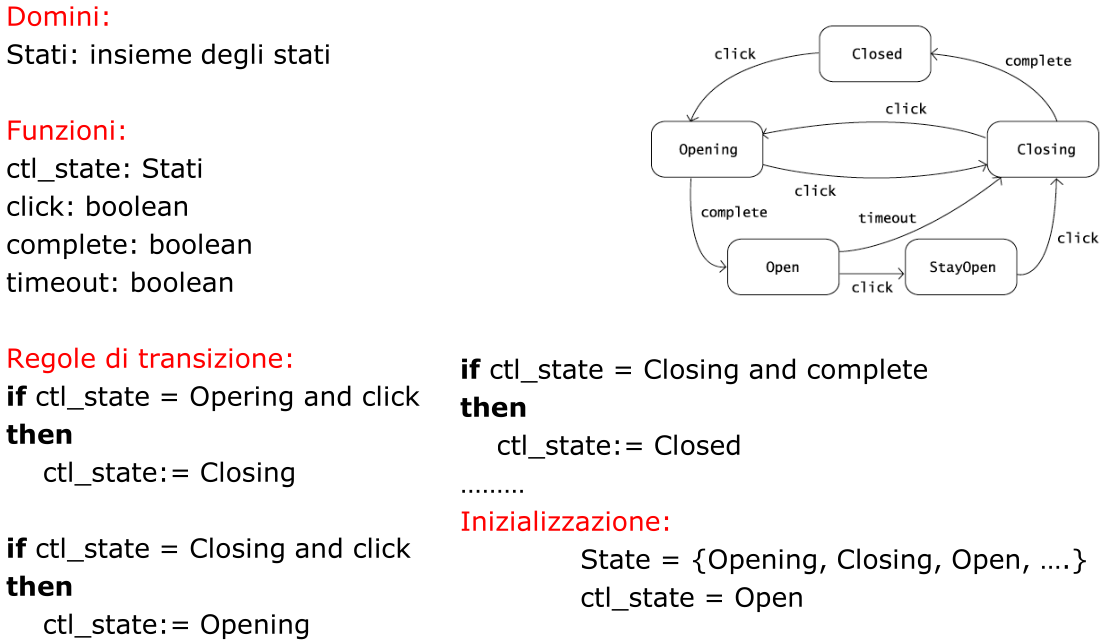
\includegraphics[width=0.92\linewidth]{chapters/1-asm/images/fsm-asm2.png}
\end{figure}

\noindent Possiamo definire ASM = (header, body, main rule, inizialization)

\begin{figure}[H]
    \centering
    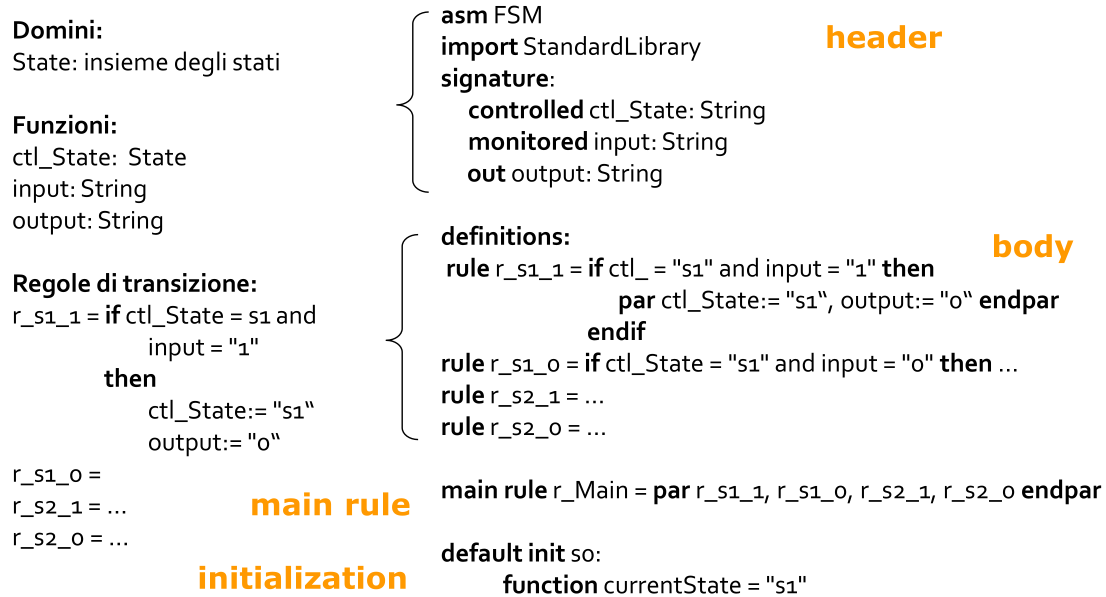
\includegraphics[width=0.92\linewidth]{chapters/1-asm/images/comp-asm.png}
\end{figure}

\section{Formalismo}

\subsection{Vocabolario}
\underline{\textbf{DEF:}} Un \textbf{vocabolario} $\Sigma$ è una collezione finita di nomi di 
funzioni.

\noindent Le funzioni possono essere dinamiche o statiche, a seconda che l'interpretazione 
del nome della funzione cambia o no da uno stato al successivo (funzioni 
in senso matematico).

\subsection{Costanti}
Le funzioni statiche di arietà zero sono dette \textbf{costanti}. Ogni 
vocabolario contiene sempre le costanti \textit{undef, true, false}.

\noindent Ad esempio:
\begin{itemize}
    \item i numeri sono costanti numeriche
    \item \texttt{voto = 30}
\end{itemize}


\subsection{Funzioni statiche}
Le funzioni statiche (arietà $>0$) sono definite tramite una legge fissa.

\noindent Ad esempio:
\begin{itemize}
    \item operazioni tra numeri (+, -, \dots)
    \item operazioni tra booleani (AND, OR, \dots)
    \item \texttt{max(m, n)}
\end{itemize}

\subsection{Fuzioni dinamiche}
Le funzioni dinamiche di arietà zero sono le variabili dei linguaggi 
di programmazione.

\subsection{Stato ASM}
\underline{\textbf{DEF:}} Fissato un vocabolario $\Sigma$, uno \textbf{stato} A del 
vocabolario $\Sigma$ è un insieme non vuoto $X$, detto \textit{superuniverso di A}, con 
le interpretazioni dei nomi delle funzioni di $\Sigma$.

\noindent Da questa definizione, segue che:
\begin{itemize}
    \item se $f$ è un nome di funzione \textit{n-aria} di $\Sigma$, allora 
    la sua interpretazione $f^A$ è una funzione da $X^n$ a $X$
    \item Se $c$ è un nome di costante di $\Sigma$, allora la sua interpretazione $c^A$ è un elemento di $X$
\end{itemize}

\noindent Possiamo definire il superuniverso come un \textit{"dominio di 
interpretazione"}; i simboli del vocabolario, presi singoralmente, sono soltanto simboli.

\subsection{Domini ASM}
Il superuniverso di uno stato ASM è suddiviso in \textit{universi}, 
rappresentati dalle loro funzioni caratteristiche.

\begin{center}
    \textit{Se A è un sottoinsieme dell'insieme X, la funzione caratteristica di A è quella 
    funzione da X all'insieme $\{0 , 1\}$ che sull'elemento x $\in$ X vale 1 se x appartiene ad A, e vale 0 in caso contrario.  }
\end{center}

\noindent Ogni universo rappresenta un dominio. In base a questa 
rappresentazione degli insiemi in termini di funzioni caratteristiche, uno stato di una 
ASM consente di modellare \textbf{domini eterogenei}.

\noindent Alcuni esempi di domini:
\begin{itemize}
    \item predefiniti, come \texttt{Interi, String, \dots}
    \item definiti dall'utente, come tipi astratti o a partire da altri domini
\end{itemize}

\subsubsection{Esempio}
Dominio $X=\{1,2,a,b,mario,pippo\}$, ripartito in domini:
\begin{itemize}
    \item $Interi = \{1.2\}$
    \item $Char = \{a,b\}$
    \item $String = \{mario, pippo\}$
\end{itemize}

\subsection{Termini ASM}
\underline{\textbf{DEF:}} i termini di $\Sigma$ sono espressioni sintattiche così costruite:
\begin{enumerate}
    \item Variabili $v_0, v_1, v_2, \dots$ sono termini 
    \item Costanti $c$ di $\Sigma$ sono termini 
    \item Se $f$ è un nome di funzione \textit{n-aria} di $\Sigma$ e 
    $t_1, \dots, t_n$ sono termini 
    
    $\Rightarrow f(t1, \dots, t_n)$ è un termine 
\end{enumerate}

\noindent Ad esempio:
\begin{itemize}
    \item $v_0 + v_1$
    \item $1 + (v_2 * 0)$
\end{itemize}

\noindent Un termine che non contiene variabili è detto chiuso. I termini 
sono \textit{oggetti sintattici}. \textbf{Assumono significato (o semantica)
nello stato}; il suo valore è l'\textit{interpretazione del termine} in $A$.



\chapter{Prime tecniche di analisi}
\section{Analisi di un modello}
Per l'analisi di un modello si usano due approcci:
\begin{itemize}
    \item \textbf{Validazione:} necessaria per controllare che il
    sistema soddisfi i requisiti richiesti
    \item \textbf{Verifica:} necessaria per garantire proprietà
    (safety, leaveness, assenza deadlock,
    reachability, ecc.)
\end{itemize}
La validazione dovrebbe precedere la verifica per individuare errori il prima possibile
e evitare di provare proprietà corrette su specifiche incorrette.

\noindent Sono possibili due prime forme di analisi
sul ground model:
\begin{itemize}
    \item Garanzia degli invarianti
    \item Validazione tramite scenari
\end{itemize}

\subsection{Garanzia degli invarianti}
In un modello ASM gli \textit{invarianti} sono usati per esprimere \textbf{vincoli} su funzioni e/o regole
che devono essere garantiti in ogni stato. 

\noindent In programmi AsmetaL usare gli invarianti è utile per scoprire errori di modellazione
In generale, l'assenza di violazione di invarianti non può essere considerata una prova della correttezza del modello, mentre la violazione di
assiomi, è prova della incorrettezza del modello

\noindent Dochiarazione degli invarianti:
\begin{itemize}
    \item Gli invarianti vanno dichiarati subito prima della main rule
    \item Ogni invariante è dichiarato mediante la keyword \textit{invariant} che precede il nome attribuito all'assioma
    \item Le funzioni e regole su cui è espresso il vincolo vanno listate dopo la keyword \textit{over}
\end{itemize}

\begin{figure}[H]
    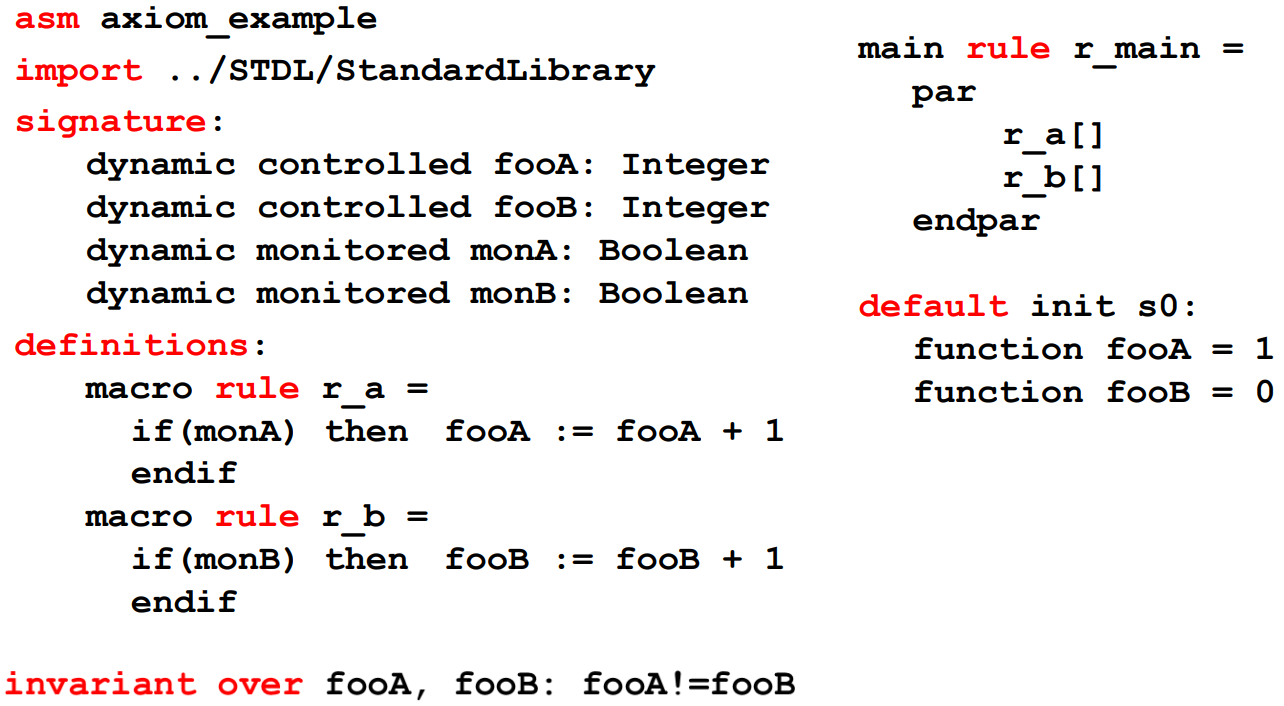
\includegraphics[width=0.8\linewidth]{chapters/2/images/axiomex.png}
\end{figure}


\subsection{Validazione tramite scenari}
\begin{itemize}
    \item \textbf{Tecniche:} Generazione di scenari, sviluppo di prototipi, animazione, simulazione, testing 
    \item \textbf{Scenario:} descrizione di un possibile comportamento del sistema (interazione osservabile tra il sistema ed il suo
    ambiente in specifiche situazioni)
\end{itemize}

\noindent Gli scenari sono costituiti attraverso una notazione testuale (Avalla)
Semantica chiara (definita in termini di ASM) e capacità di descrivere anche dettagli interni (non solo black box come per UML use cases, ma
anche informazioni sullo stato).

\subsubsection{Da attore UML  a attore ASM}
\noindent Nell'UML use case l'attore interagisce col sistema, uno o più scenari possono essere generati per
ogni caso d'uso, però visione BLACK BOX.
\noindent L'ASM Observer può verificare lo stato interno della macchina e gli invarianti, e
richiede l'esecuzione di regole arbitrarie.

\begin{figure}[H]
    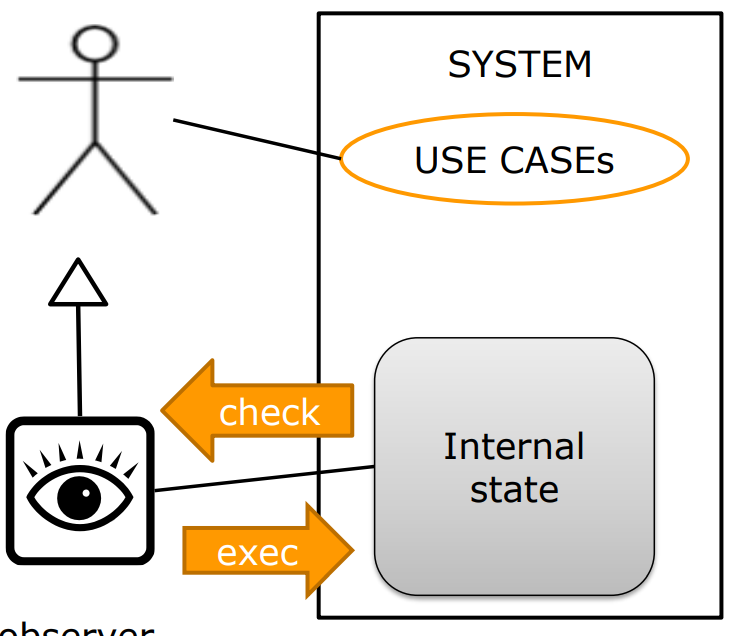
\includegraphics[width=0.5\linewidth]{chapters/2/images/attoreASM.png}
\end{figure}

\subsubsection{Doppio uso degli scenari}
\begin{itemize}
    \item Due tipi di attori esterni:
    \item \begin{itemize}
        \item \textbf{User:} ha una visione \textit{black box} del sistema
        \item \textbf{Observer:} ha una visione \textit{grey box}
    \item Due obiettivi per gli scenari:
    \item \begin{itemize}
        \item \textbf{Validazione classica:} azione dell'utente e reazioni della macchina
        \item \textbf{Attività di testing:} ispezione dell’observer dello stato interno
        della macchina
    \end{itemize}
    \end{itemize}
\end{itemize}

\subsubsection{Scenario ASM}
Sequenza di interazione consentite delle azioni:
\begin{itemize}
    \item da parte di user/observer: 
    \begin{itemize}
        \item \textbf{set} the environment (i.e. the values of
        monitored/shared functions)
        \item \textbf{check} for the machine outputs (i.e. the values of
        out functions)
        \item \textbf{check} the machine state and invariants
        \item \textbf{ask} for the execution of given transition rules
    \end{itemize}
    \item da parte della macchina: 
    \textbf{makes} one \textit{step} as reaction of the actor actions
\end{itemize}

\subsubsection{Primitive di AvValLa - Asm Validation Language}
\begin{figure}[H]
    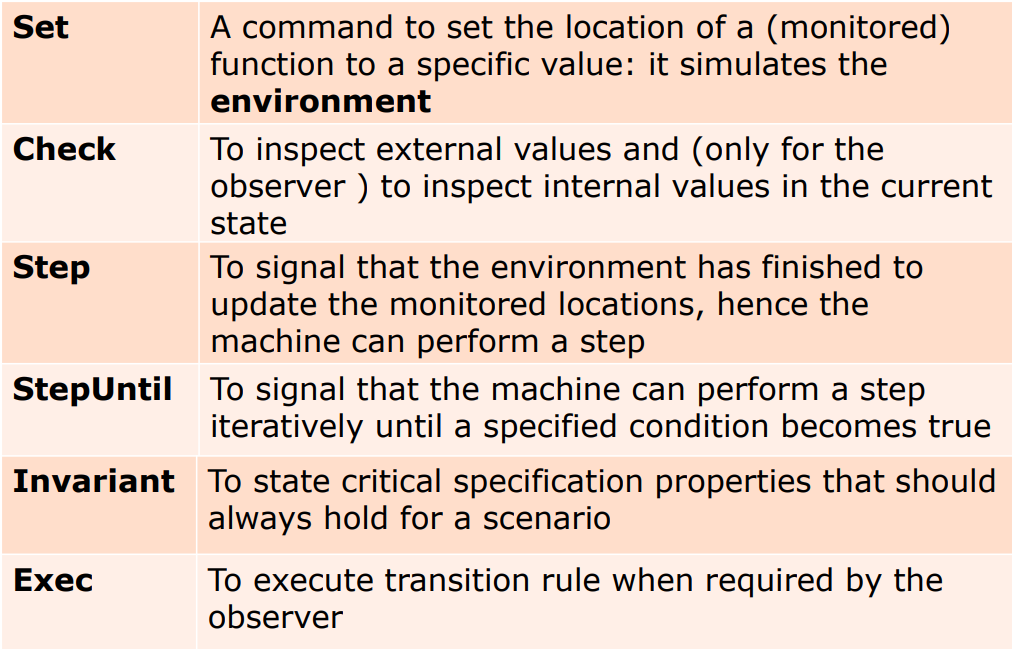
\includegraphics[width=0.8\linewidth]{chapters/2/images/Avalla.png}
\end{figure}

\subsubsection{Sintassi Avalla}
\begin{figure}[H]
    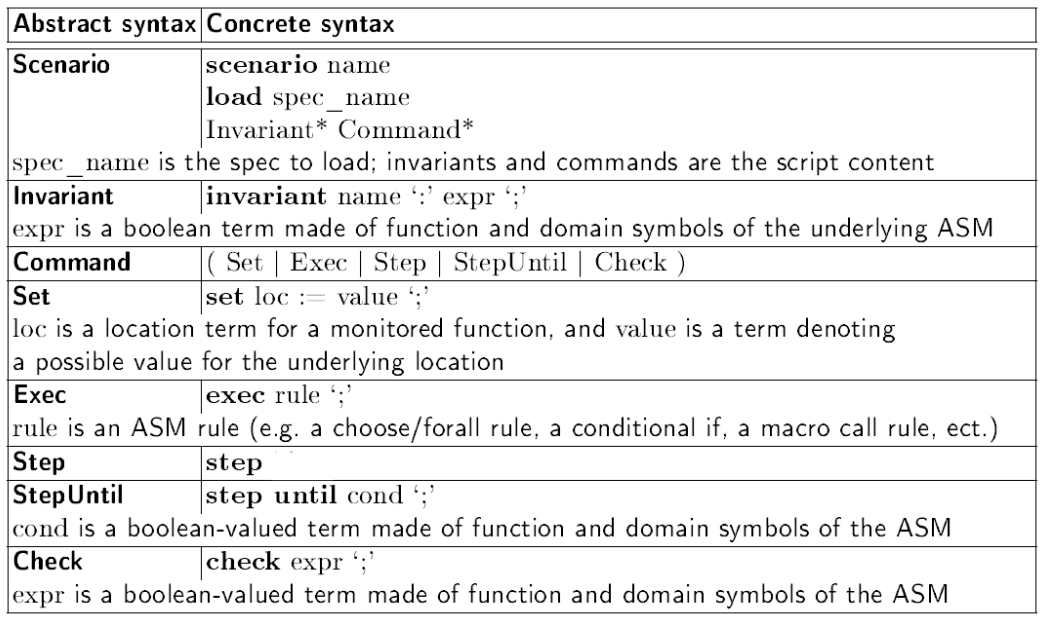
\includegraphics[width=0.8\linewidth]{chapters/2/images/sintassiAvalla.png}
\end{figure}



\chapter{Composizione di modelli: ASM multi agenti}
\noindent Grazie alle regole per la strutturazione, è possibile definire un sistema distribuito
come una composizione di ASM.
\begin{itemize}
    \item Ogni componente del sistema distribuito viene
    modellato mediante una opportuna ASM
    \item Risulta un sistema di ASM Distribuite, dette anche \textbf{ASM multi agenti}
\end{itemize}

\section{ASM multi agenti}
\noindent Descrivono un modello distribuito della computazione. La computazione distribuita è modellata
mediante un insieme di Agenti che operano in modo concorrente
\begin{itemize}
    \item \textit{Movimenti} concorrenti sincroni/asincroni
    \item \textit{Stati globali} condivisi tra gli agenti
\end{itemize}

\noindent Gli agenti ASM:
\begin{itemize}
    \item Possono essere creati dinamicamente
    \item Hanno una visione parziale dello stato globale
    \item Hanno il proprio programma da eseguire
\end{itemize}

\noindent Le ASM multi agenti sono classificate in:
\begin{itemize}
    \item \textbf{Sincrone:} gli agenti eseguono il loro programma in parallelo, sincronizzati su un implicito clock globale del sistema
    \item \textbf{Asincrone:} gli agenti eseguono il loro programma in parallelo, ma in modo indipendente tra loro 
    \begin{itemize}
        \item Ciascuno ha il \textit{proprio clock} che regola la durata du una mossa
        \item Ciascuno opera nel \textit{proprio stato locale}
    \end{itemize}
\end{itemize}

\subsection{Definizione ASM multiagente:}
\noindent 
\begin{center}
    \textit{Una sync/async ASM è un insieme di coppie (a, ASM(a)) dove
    \begin{itemize}
        \item di agenti a $\in$ Agent (il dominio degli agenti)
        \item e programmi ASM(a) che sono ASM di base
    \end{itemize}}
\end{center}

\subsection{Codifica AsmetaL di ASM Multiagenti}
\begin{center}
    $[asyncr] asm ASM-name$
\end{center}
\noindent a parola chiave asyncr è opzionale(perchè racchiusa nelle parentesi quadre)
\begin{itemize}
    \item Se presente, denota una ASM \textit{asincrona} multi-agent
    \item Se omessa, l’ASM è considerata \textit{sincrona} multi-agent
\end{itemize}

\begin{itemize}
    \item Ogni agente ha una \textit{visione parziale} dello stato globale
    \begin{itemize}
        \item \textit{View(a, M)} indica la vista dell’agente a dello
        stato globale di una ASM M
    \end{itemize}
    \item Ogni agente può avere una \textit{visione privata} non condivisa con altri agenti
    \begin{itemize}
        \item per una $f : A-> B$ globale, la dichiarazione privata di f diventa $ f : Agent$ x $A->B$ 
        \begin{itemize}
            \item f(self,x) denota la \textit{verisone privata di f(x)} dell'agente corrente \textit{self}
        \end{itemize}
        \item \textit{self} viene interpretata da \textit{a} (agente) come se stesso
    \end{itemize}
\end{itemize}


\chapter{Specifica di protocolli di sicurezza: il protocollo di Needham Schroeder}
\section{Crittografia: concetti base}
\begin{itemize}
    \item \textbf{Algoritmi crittografici:} algoritmi che trasformano un testo (o una info) in un testo cifrato utilizzando chiavi
    \item \textbf{Protocolli crittografici:} sequenze di scambio di messaggi a cui gli agenti possono applicare
    algoritmi crittografici
    \begin{itemize}
        \item \textbf{a chiave simmetrica:} la stessa K è utilizzata per criptare e decriptare
        \item \textbf{a chiave pubblica:} K-pub per criptare e K-priv per decriptare
        \item \textbf{a chiave condivisa:} una K-AB tra 2 agenti fornita da un terzo
    \end{itemize}
\end{itemize}

\subsubsection{Protocolli per l'autenticazione}
\noindent Lo scopo è \textbf{l'autenticazione}
\begin{itemize}
    \item fornire ad una parte la certezza dell'identità del mittente del messaggio ricevuto 
    \item eventualmente stabilire una chiave (o altra info) comune 
\end{itemize}

\noindent \textbf{Segretezza:} in più possono garantire che l'informazione (o parte) scambiata è rimasta segreta

\subsubsection{Assunzioni di base}
\begin{itemize}
    \item \textbf{Forza della spia:} la spia (man in the middle) può
    \begin{itemize}
        \item intercettare (ed eventualmente analizzare) ogni messaggio che sia stato spedito da un agente
        \item formare (sintetizzare) nuovi messaggi utilizzando la sua base di conoscenze
        \item cambiare destinatario di un messaggio
    \end{itemize}
    \item \textbf{Forza della crittografia:} 
    \begin{itemize}
        \item un messaggio può essere decriptato solo se si ha la chiave giusta
        \item un agente può generare sempre nonces nuove
        \item un agente autenticato è non compromesso se la sua chiave privata non è nota alla spia
    \end{itemize}
\end{itemize}

\section{Needham-Schroeder a chiavi pubbliche}
\noindent \textbf{Obiettivo:} stabilire mutua autenticazione tra due agenti A e B (e una nonce segreta comune)
\subsubsection{Protocollo}
\begin{enumerate}
    \item \textbf{A} che vuole iniziare la comunicazione con \textbf{B}, manda una nuova nonce a \textbf{B}:
    \begin{center}
        $A->B :$ \{Na, A\}Kb
    \end{center}
    \item \textbf{B} legge il messaggio, rimanda la nonce di \textbf{A} più un'altra nuova:
    \begin{center}
        $B->A :$ \{Na, Nb\}Ka
    \end{center}
    \item \textbf{A} legge il messaggio, riconosce la nonce rispedita da \textbf{B} (solo B può averla letta) e rimanda a \textbf{B}, Nb:
    \begin{center}
        $A->B :$ \{Nb\}Kb
    \end{center}
    \item \textbf{B} ricevendo indietro la nonce Nb sa che l'autenticazione (handshake) è avvenuta (solo \textbf{A} può averla letta)
\end{enumerate}

\subsubsection{Vulnerabilità}
\noindent Il protocollo è suscettibile ad attacchi di tipo \textit{man in the middle}:
\begin{itemize}
    \item un impostore Spy riesce ad avere il controllo del traffico (modellato con Alice che inizia una sessione di comunicazione con Spy)
    \item inoltra i messaggi a Bob convincendolo di essere in comunicazione con Alice ed inganna Alice facendole credere di comunicare con Bob     
\end{itemize}

\noindent Spy agisce da "uomo nel mezzo" e intercetta tutti i messaggi di Bob, che crede di essere in
comunicazione sicura con Alice

\noindent L'attacco è stato descritto per la prima volta da Gavin Lowe nel 1995

\subsection{Attacco di Lowe}
\noindent \textbf{A} inizia una istanza del protocollo con la spia (o con un agente compromesso)
\begin{center}
    $A-> Spy :$ \{Na, A\}Ks
    
    $Spy->B :$ \{Na, A\}Kb
    
    $B->A :$ \{Na, Nb\}Ks
    
    $Spy->B :$ \{Nb\}Kb
\end{center}

\noindent La spia acquisisce una informazione segreta di B: \textbf{Nb è compromessa}

\noindent A sta usando una nonce compromessa

\noindent B ha una nonce Nb compromessa, eppure né A né B sono compromessi

\noindent Per garantire l'autenticazione il protocollo richiederebbe
\begin{itemize}
    \item che gli agenti non siano compromessi ma
    \item anche che non abbiano iniziato comunicazioni
    con agenti compromessi
\end{itemize}

\subsubsection{La soluzione di Lowe}
\begin{enumerate}
    \item \textbf{A} che vuole iniziare la comunicazione con \textbf{B}, manda una nuova nonce a \textbf{B}:
    \begin{center}
        $A->B :$ \{Na, A\}Kb
    \end{center}
    \item \textbf{B} legge il messaggio, rimanda la nonce di \textbf{A} più un'altra nuova e \underline{\textbf{la sua identità}}:
    \begin{center}
        $B->A :$ \{Na, Nb, B\}Ka
    \end{center}
    \item \textbf{A} legge il messaggio, riconosce la nonce rispedita da \textbf{B} (solo B può averla letta) e rimanda a \textbf{B}, Nb:
    \begin{center}
        $A->B :$ \{Nb\}Kb
    \end{center}
    \item \textbf{B} ricevendo indietro la nonce Nb sa che l'autenticazione è avvenuta (solo \textbf{A} può averla letta)
\end{enumerate}

\subsubsection{Esercizio NS in ASM}

\end{document}